\documentclass[10pt,twocolumn]{article}
	
\usepackage{myfontstyle}
\usepackage{mypackages}
\usepackage{mymacros}
\usepackage{mycommands}
\usepackage{graphicx}
\usepackage{hyperref}
\usepackage{listings}
\usepackage{xcolor}


%%% This defines a style for code blocks (listings package) ----------------
\definecolor{codegreen}{rgb}{0,0.6,0}
\definecolor{codegray}{rgb}{0.5,0.5,0.5}
\definecolor{codepurple}{rgb}{0.58,0,0.82}
\definecolor{backcolour}{rgb}{0.95,0.95,0.92}

\lstdefinestyle{mystyle}{
    backgroundcolor=\color{backcolour},   
    commentstyle=\color{codegreen},
    keywordstyle=\color{magenta},
    numberstyle=\tiny\color{codegray},
    stringstyle=\color{codepurple},
    basicstyle=\ttfamily\footnotesize,
    breakatwhitespace=false,         
    breaklines=true,                 
    captionpos=b,                    
    keepspaces=true,                 
    numbers=left,                    
    numbersep=5pt,                  
    showspaces=false,                
    showstringspaces=false,
    showtabs=false,                  
    tabsize=2
}

\lstset{style=mystyle}

%%%----------------------------------------

\begin{document}
\thispagestyle{fancy1}

%%% Title and Abstract------------------------
\twocolumn[
\begin{center}
	\hrule
	\vspace{3pt}
	% Title:
	{\sffamily\bfseries\Large
		Report for Laboratory 6: Realizing a Discrete Dynamic System
	} \\
	{\color{gray}
		\vspace{3pt}
		\hrule
		\vspace{3pt}
	}
	{
		\hspace*{\fill}
		Julian Soh
		\hspace*{\fill}
%		Second Author
%		\hspace*{\fill}
%		Third Author
%		\hspace*{\fill}
%		Fourth Author    % uncomment these two lines if there's a fourth author
%		\hspace*{\fill}
	}\\
	\vspace{3pt}
	{\itshape
		\hspace*{\fill}
		Department of Mechanical Engineering, Saint Martin's University
		\hspace*{\fill} \\
		\hspace*{\fill}
		ME/EE 477---Embedded Real-Time Computing for Mechanical Engineers
		\hspace*{\fill}
	}\\
	\vspace{3pt}
	{
		\hspace*{\fill}
		\today{} % today's date ... can type manually instead
		\hspace*{\fill}
	}
	\vspace{3pt}
	{\color{gray}\hrule}
%	\vspace{2pt}
\end{center}
% Abstract:
\begin{adjustwidth}{1.5in}{1.5in}
{\small
\noindent\textbf{Abstract.} \hspace{1em}
Writing a program capable of approximating the performance of any SISO (Single Input, Single Output), LTI (Linear Time-Invariant) system.
Program will use interrupts (see Lab 5) to read the analog input connector of the MyRio that is connected to a function generator, convert the
signal from Analog to Digital (ADC), approximate the system's performance and write that to the output of the Digital to Analog (DAC) converter on the MyRio.
}
\end{adjustwidth}
\vspace{9pt}
\hrule
\vspace{1\baselineskip}
]

%%% Body -------------------------

\section{Introduction} 
\label{sec:introduction}
In this laboratory exercise, we developed a general-purpose program to approximate the behavior of any SISO (single-input, single-output), linear time-invariant (LTI) system. The implementation is based on a discrete-time difference equation, allowing the program to emulate a wide range of transfer-function-based system dynamics.

The objectives of this lab were:
\begin{enumerate}
	\item To use real-time clock interrupts for timing control
	\item To implement an arbitrary transfer function generator
	\item To incorporate analog-to-digital and digital-to-analog conversion
\end{enumerate}

\section{Materials and Methods}

\subsection{Materials}
The materials used in this experiment were:
\begin{itemize}
	\item Windows 10 computer with myRIO support for C and Eclipse IDE.
	\item NI myRIO-1900
	\item Rigol DHO914S Digital Oscilloscope with $25 Mhz$ function generator
\end{itemize}

\subsection{Main Function Implementation}
The software architecture uses two concurrent execution paths: a \texttt{main()} routine and an interrupt service routine (ISR) running in a dedicated thread. The timer interrupt drives the ISR at a fixed sampling period of $0.5\,\text{ms}$, while the ISR updates the DAC output from the ADC input through a difference-equation-based model.

The \texttt{main()} function is intentionally minimal and is responsible for control flow only:
\begin{enumerate}
	\item Configure and enable the timer interrupt request (Timer IRQ).
	\item Remain in a polling loop until the keypad returns \texttt{a} using \texttt{getkey()} (implemented previously in Lab 3).
	\item Request ISR-thread shutdown by clearing the \texttt{irqThreadRdy} run flag, then block until the ISR thread exits cleanly.
\end{enumerate}

\subsection{Interrupt Service Routine (ISR) Thread}
The ISR thread realizes the discrete dynamic system in real time. Its core logic runs inside a \texttt{while} loop that repeatedly checks \texttt{irqThreadRdy}; the loop continues while the flag indicates that execution should proceed.

Before entering the loop, the analog I/O subsystem is initialized and analog output connector C channel 1 (AOC1) is forced to $0\,\text{V}$.

For each interrupt cycle, the ISR performs the following sequence:
\begin{enumerate}
	\item Wait for the next IRQ event, then program the timer for the next interval by writing BTI to \texttt{IRQTIMERWRITE} and asserting \texttt{TRUE} on \texttt{IRQTIMERSETTIME}.
	\item Acquire the current sample $x(n)$ from analog input connector C channel 0 (AIC0).
	\item Compute the current output $y(n)$ by invoking \texttt{cascade()}, which evaluates all biquad stages using the section-by-section difference-equation form.
	\item Send $y(n)$ to analog output connector C channel 1 (AOC1).
	\item Acknowledge the interrupt so the next cycle can be serviced.
\end{enumerate}

After shutdown, the thread writes the measured response data to \texttt{Lab6.mat}.

The ISR allocates and manages the data required by the dynamic model, including:
\begin{enumerate}
	\item BTI duration in microseconds.
	\item Number of biquad sections, $n_s$.
	\item Section coefficients ($a_k$ and $b_k$) and the stored prior input/output samples.
\end{enumerate}

To keep the cascade manageable, each biquad stage is represented by a structure that stores its coefficients and state history. This makes the full multi-section system easier to configure, evaluate, and maintain.

\section{Laboratory Exploration and Evaluation}

\subsection{Problem L6.1}
Write the \texttt{main()} program described in Section L6.2, including the timer ISR, but do not implement \texttt{cascade()} yet. Instead, complete and debug everything else in the framework for the biquad-cascade implementation. Set up \texttt{main()} and the ISR with the required arrays and timing. In the ISR, pass the ADC input directly to the DAC output:

\begin{lstlisting}[language=C]
VADin = Aio_Read(&AIC0);
Aio_Write(&AOC1, VADin);
\end{lstlisting}

Use this direct pass-through mode to view input and output on the oscilloscope and verify that interrupt timing is operating correctly.

\vspace{\baselineskip}
The full program is available at \url{https://github.com/juliansoh/ME477/blob/main/workspace/Julian_lab6/main.c}.

The input-to-output pass-through behavior was observed on the oscilloscope, as shown in \autoref{fig:Lab60}.

\begin{figure}[htb]
	\centering
	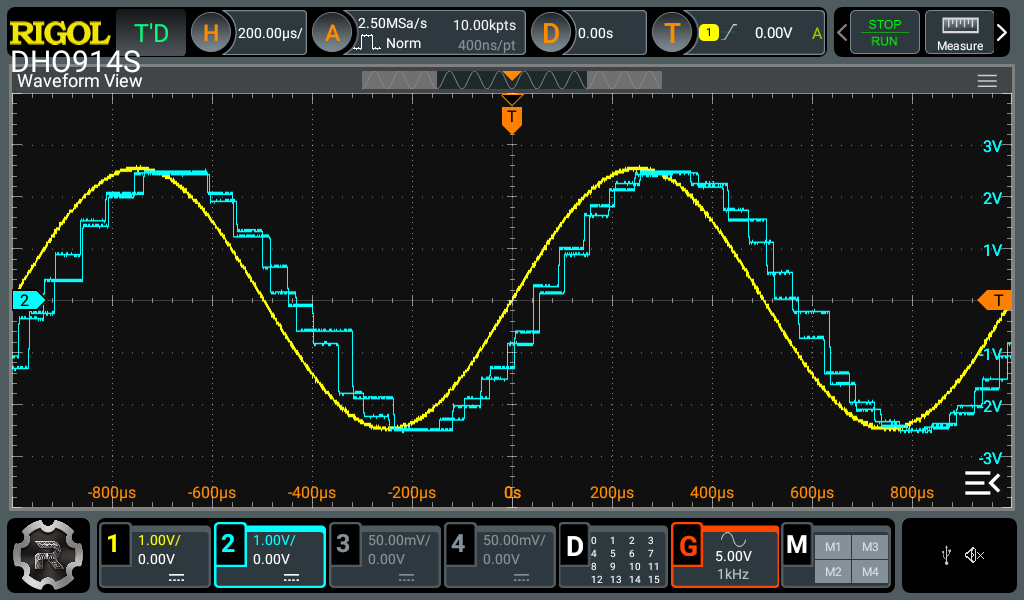
\includegraphics[width=.9\linewidth]{figures/Lab60.png}
	\caption{Oscilloscope observation for Problem L6.1 with ADC input passed directly to DAC output.}
	\label{fig:Lab60}
\end{figure}

\subsection{Problem L6.2}
Implement the \texttt{cascade()} function described in Section L6.2. Then extend the \texttt{main()} program from Problem L6.1 so that the output signal is computed through \texttt{cascade()}.

\vspace{\baselineskip}
The full program is available at \url{https://github.com/juliansoh/ME477/blob/main/workspace/Julian_lab6/main.c}.

The oscilloscope response with \texttt{cascade()} implemented is shown in \autoref{fig:Lab62}.

\begin{figure}[htb]
	\centering
	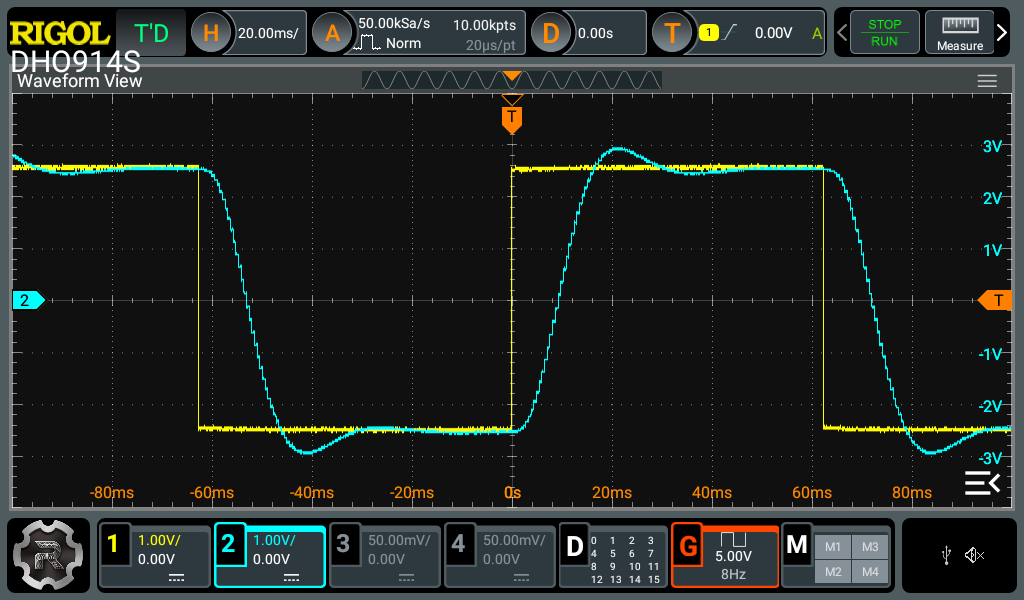
\includegraphics[width=.9\linewidth]{figures/Lab62.png}
	\caption{Oscilloscope observation for Problem L6.2 after implementing \texttt{cascade()}.}
	\label{fig:Lab62}
\end{figure}

\subsection{Problem L6.3}
Modify the timer ISR so it stores both the input and the \texttt{cascade()} output in 500-point buffers (see Appendix D.1). After the timer loop finishes, export these buffers to \texttt{Lab6.mat}.

\vspace{\baselineskip}
Instead of using MATLAB, we used Python for post-processing and analysis. Accordingly, the program was modified to capture and save the response data in CSV format.

\subsection{Problem L6.4}
Using the oscilloscope in DC coupling mode, measure the system step response by applying a low-frequency square-wave input (for example, $8\,\text{Hz}$) with $5\,\text{V}$ amplitude from the function generator.

Transfer the response data saved in \texttt{Lab6.mat} to your development computer and load it into MATLAB. Plot the measured step response and compare it with the theoretical response of the corresponding continuous-time system. MATLAB's \texttt{lsim()} can be used for the theoretical simulation.

Discuss how the measured and theoretical results differ, and explain likely causes of those differences.

\vspace{\baselineskip}
The Python post-processing code used for Problem L6.4 is available in the notebook at \url{https://github.com/juliansoh/ME477/blob/main/workspace/Julian_lab6/Reports/Lab6/data/Step-Response.ipynb}.

The oscilloscope step-response measurement was shown in \autoref{fig:Lab63}.

\begin{figure}[htb]
	\centering
	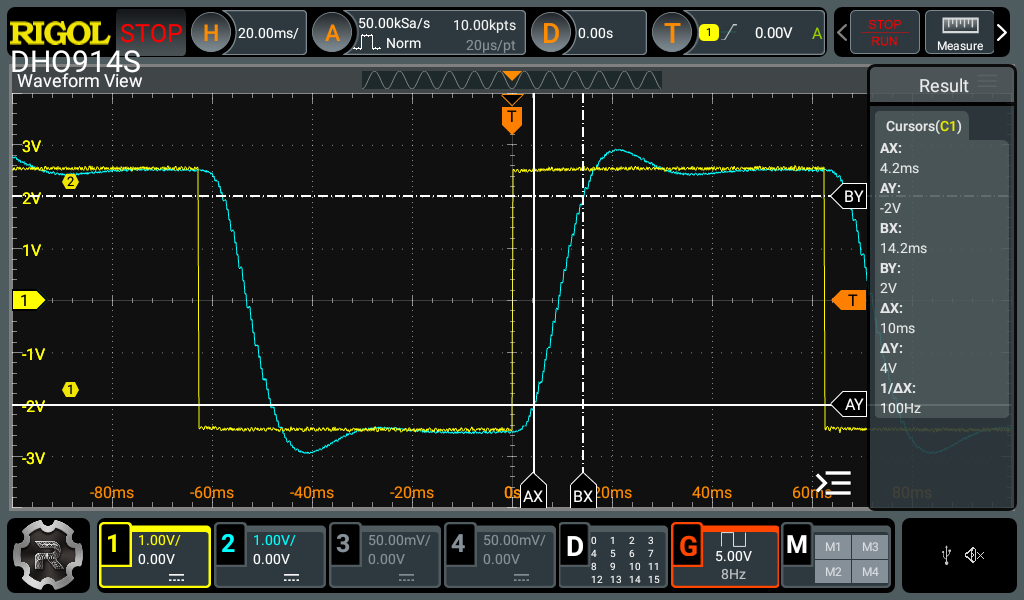
\includegraphics[width=.9\linewidth]{figures/Lab63.png}
	\caption{Oscilloscope cursor measurement for the step response in Problem L6.4.}
	\label{fig:Lab63}
\end{figure}

We used the oscilloscope cursor functions to measure the step response. The cursors were placed at Ay and By at $-2\,\text{V}$ and $+2\,\text{V}$, corresponding to the $10\%$ and $90\%$ rise-time markers, and Ax and Bx were used to measure the step time. From \autoref{fig:Lab63}, the oscilloscope showed $\Delta X = \mathbf{10\,\text{ms}}$.

The Python comparison plot of measured and theoretical step responses is shown in \autoref{fig:Lab64Python}.

\begin{figure}[htb]
	\centering
	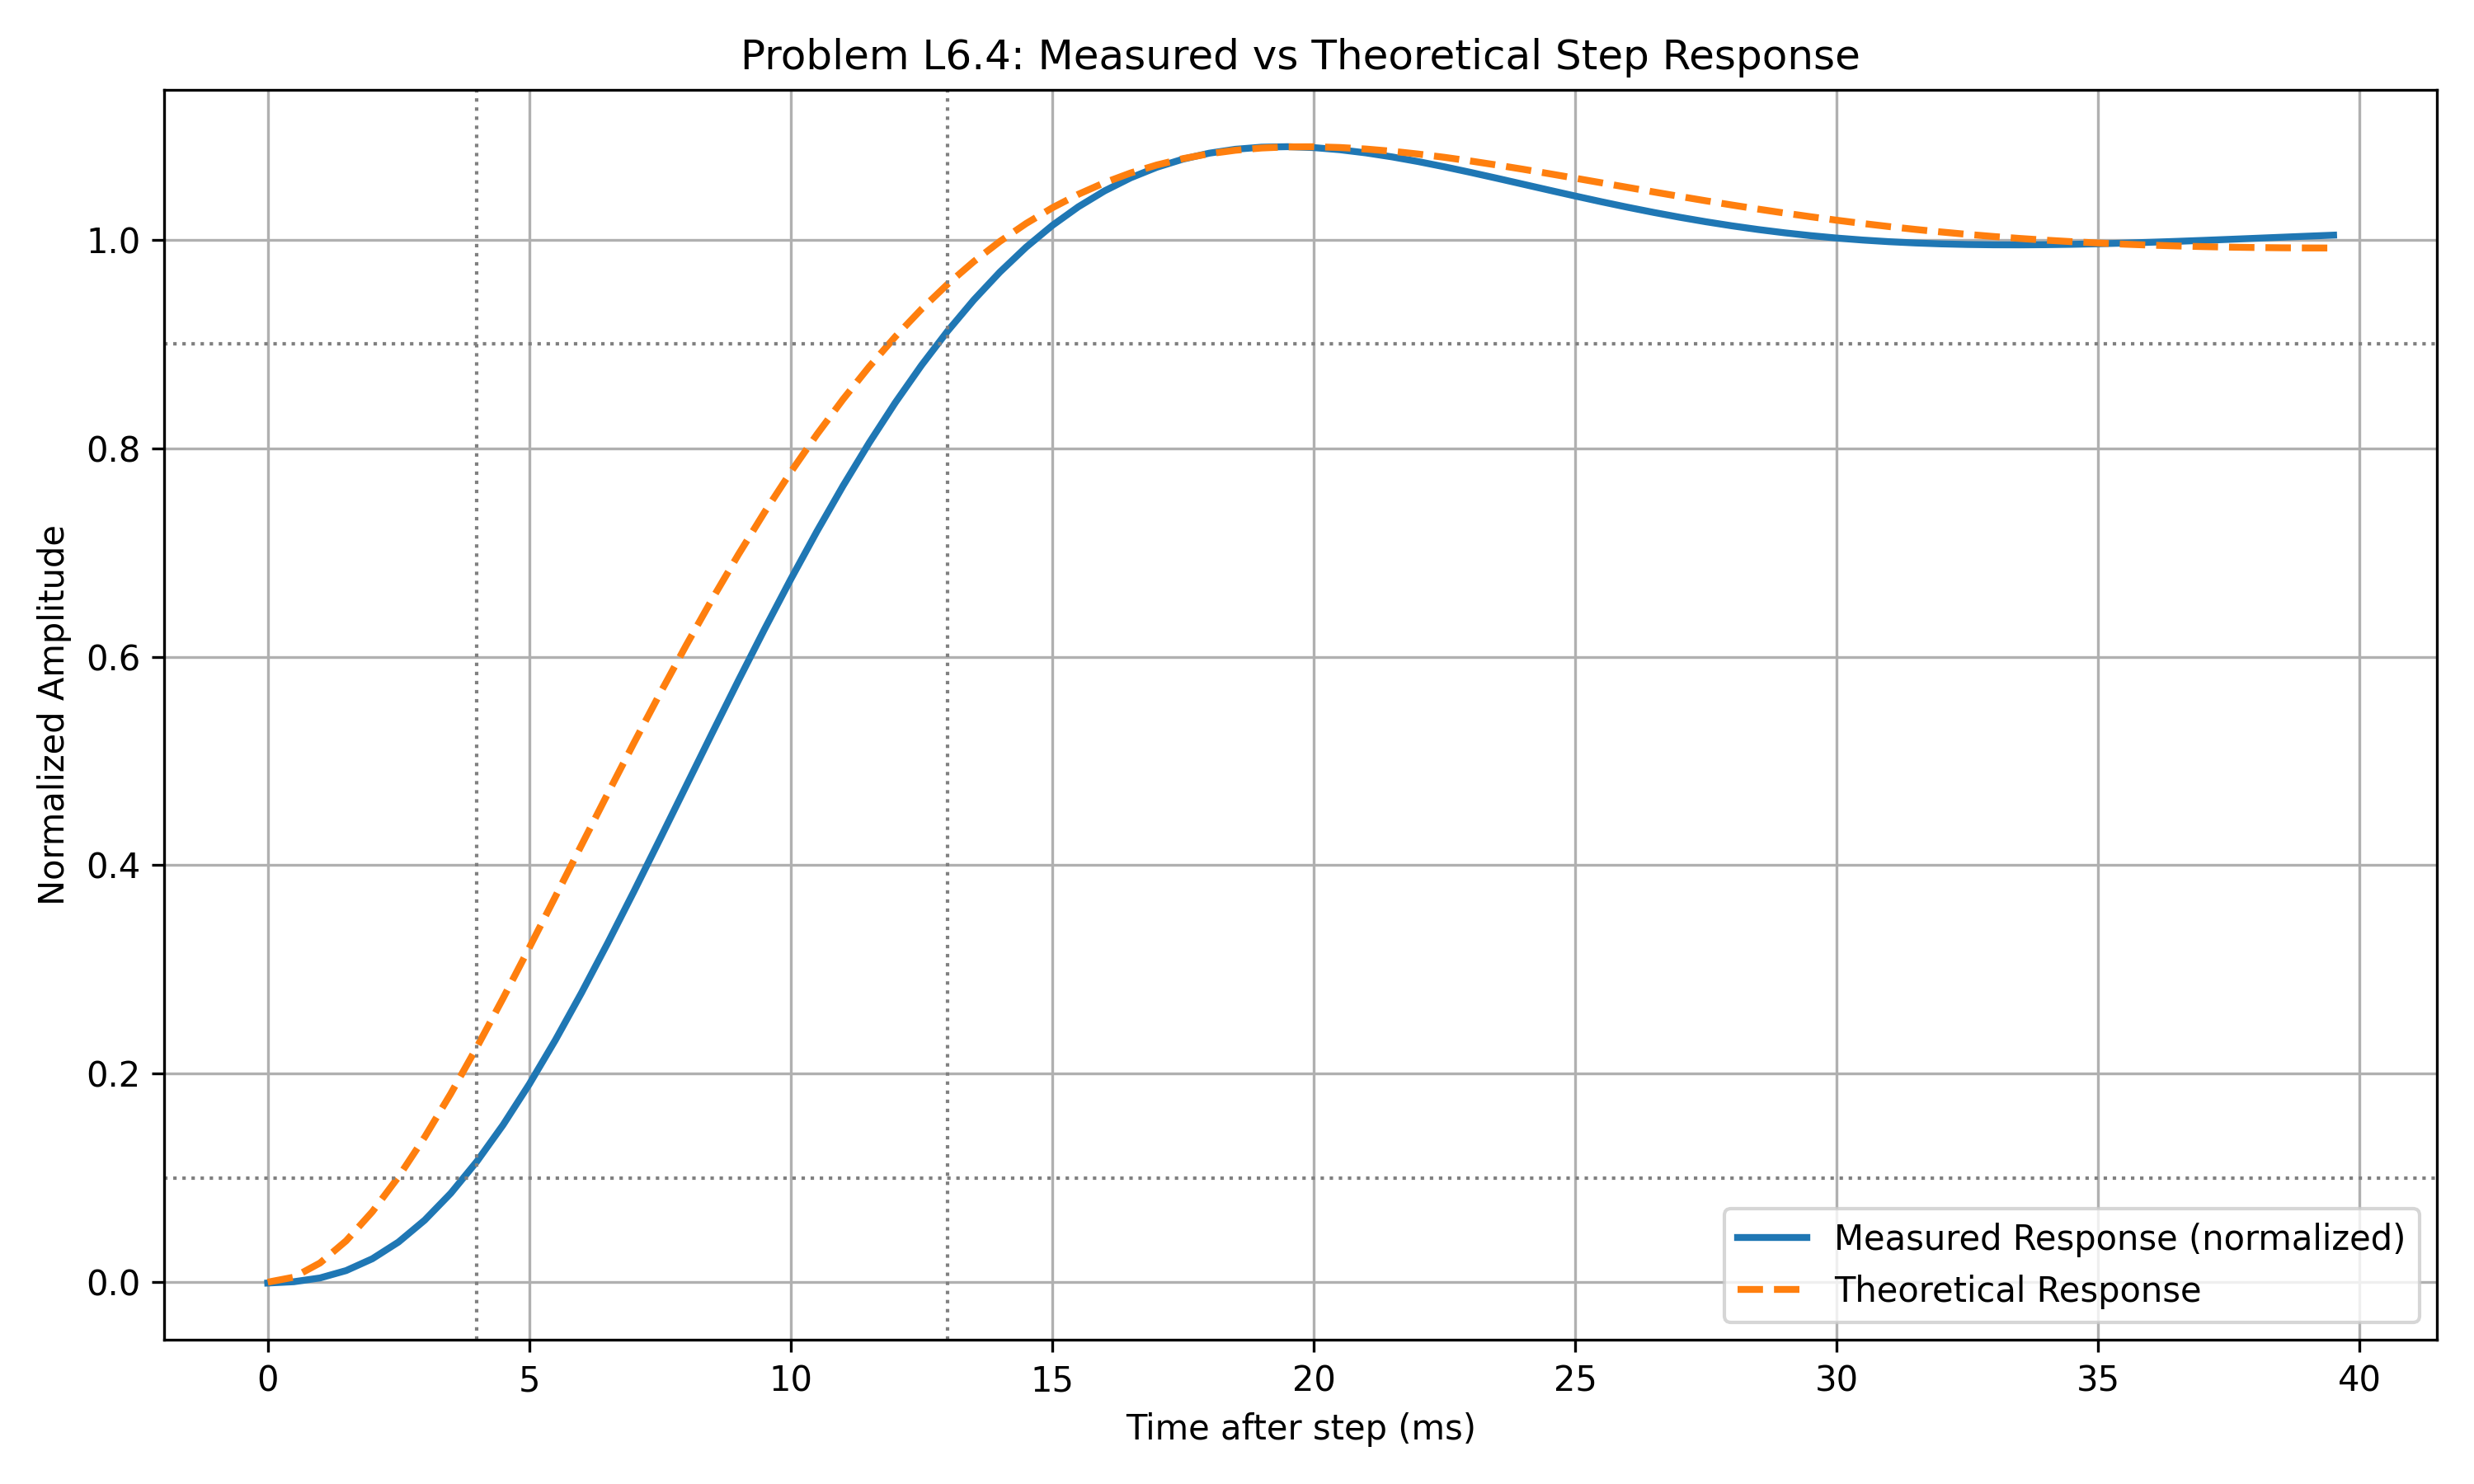
\includegraphics[width=.9\linewidth]{figures/Lab64-StepResponse-Python.png}
	\caption{Measured versus theoretical step response for Problem L6.4 (Python post-processing of \texttt{lab6.csv}).}
	\label{fig:Lab64Python}
\end{figure}

The post-processed step-response data in Python gave a measured $10\%-90\%$ rise time of approximately $9\,\text{ms}$, which is consistent with the oscilloscope cursor measurement of about $10\,\text{ms}$. A second-order continuous-time model fitted to the measured waveform produced a response that follows the overall trend well, including a small overshoot and settling behavior. However, the measured waveform is not identical to theory: the measured trace rises slightly more slowly at the beginning and shows small residual ripple/noise near the final value. These differences are expected and are mainly due to non-ideal hardware and implementation effects, including sensor/electronics noise, finite ADC resolution and sampling period, component tolerances, actuator saturation and dead-zone effects, and unmodeled dynamics that are not captured by the ideal continuous-time transfer-function model.

\subsection{Problem L6.5}
Using the oscilloscope in AC coupling mode, observe the frequency response by varying the frequency of a $5\,\text{V}$ sine-wave input.

Record the output amplitude and phase relative to the input at the following frequencies: $5$, $10$, $20$, $40$, $60$, $100$, $140$, and $200\,\text{Hz}$.

\vspace{\baselineskip}
The frequency-response measurements are shown in \autoref{fig:L65_5}, \autoref{fig:L65_10}, \autoref{fig:L65_20}, \autoref{fig:L65_40}, \autoref{fig:L65_60}, \autoref{fig:L65_100}, \autoref{fig:L65_140}, and \autoref{fig:L65_200}.

In each oscilloscope screenshot, the right-side \texttt{Result} panel is where the measured values are read:
\texttt{Vpp(C2)} for output peak-to-peak amplitude and \texttt{Phase(r-r)(C1-C2)} for phase.

\begin{table}[htb]
\centering
\caption{Measured frequency-response values from the oscilloscope in Problem L6.5.}
\label{tab:L65_measured}
\begin{tabular}{c c c}
\hline
Frequency (Hz) & \texttt{Vpp(C2)} & \texttt{Phase(r-r)(C1-C2)} \\
\hline
5   & 4.2330 V   & 15.347$^{\circ}$ \\
10  & 4.7900 V   & 32.576$^{\circ}$ \\
20  & 4.9141 V   & 67.855$^{\circ}$ \\
40  & 3.0537 V   & 154.59$^{\circ}$ \\
60  & 1.1369 V   & -156.44$^{\circ}$ \\
100 & 272.18 mV  & -119.27$^{\circ}$ \\
140 & 121.72 mV  & -127.62$^{\circ}$ \\
200 & 64.914 mV  & -150.28$^{\circ}$ \\
\hline
\end{tabular}
\end{table}

\begin{figure}[htb]
	\centering
	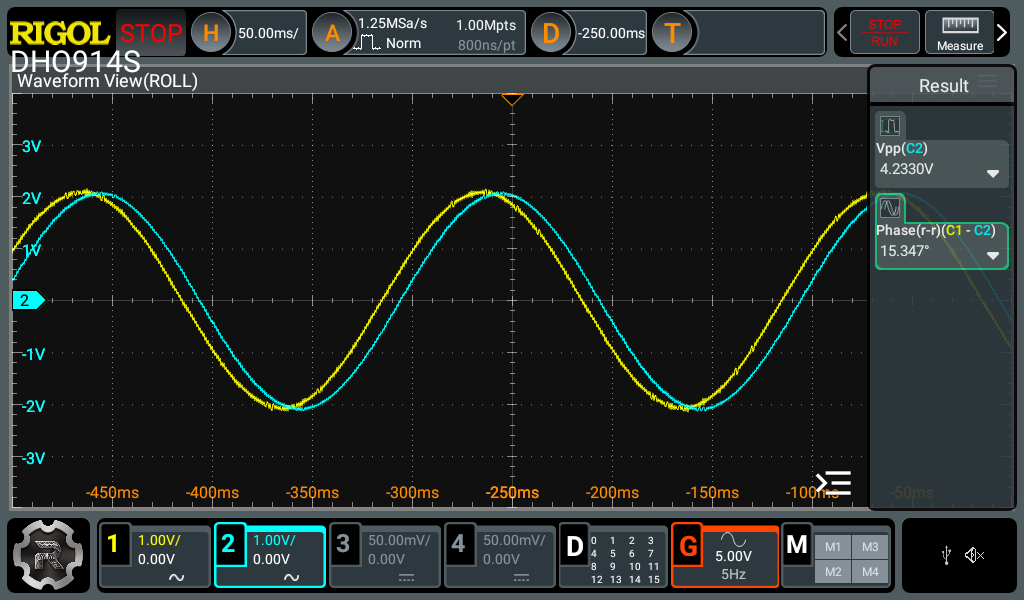
\includegraphics[width=.98\linewidth]{figures/L6_5_5Hz0.png}
	\caption{Frequency-response measurement at $5\,\text{Hz}$: \texttt{Vpp(C2)} $=4.2330\,\text{V}$, \texttt{Phase(r-r)(C1-C2)} $=15.347^{\circ}$.}
	\label{fig:L65_5}
\end{figure}

\begin{figure}[htb]
	\centering
	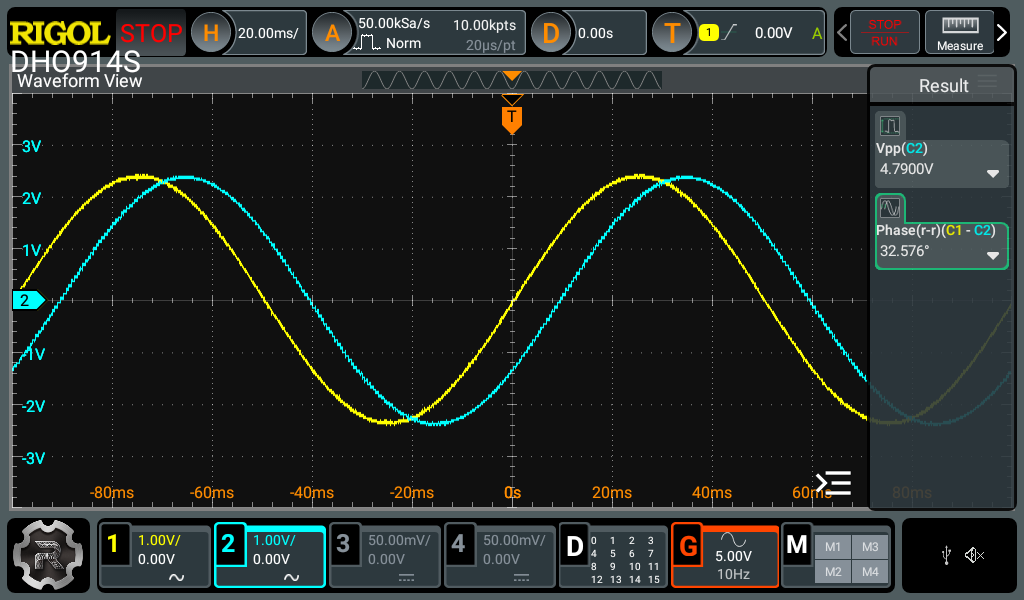
\includegraphics[width=.98\linewidth]{figures/L6_5_10Hz0.png}
	\caption{Frequency-response measurement at $10\,\text{Hz}$: \texttt{Vpp(C2)} $=4.7900\,\text{V}$, \texttt{Phase(r-r)(C1-C2)} $=32.576^{\circ}$.}
	\label{fig:L65_10}
\end{figure}

\begin{figure}[htb]
	\centering
	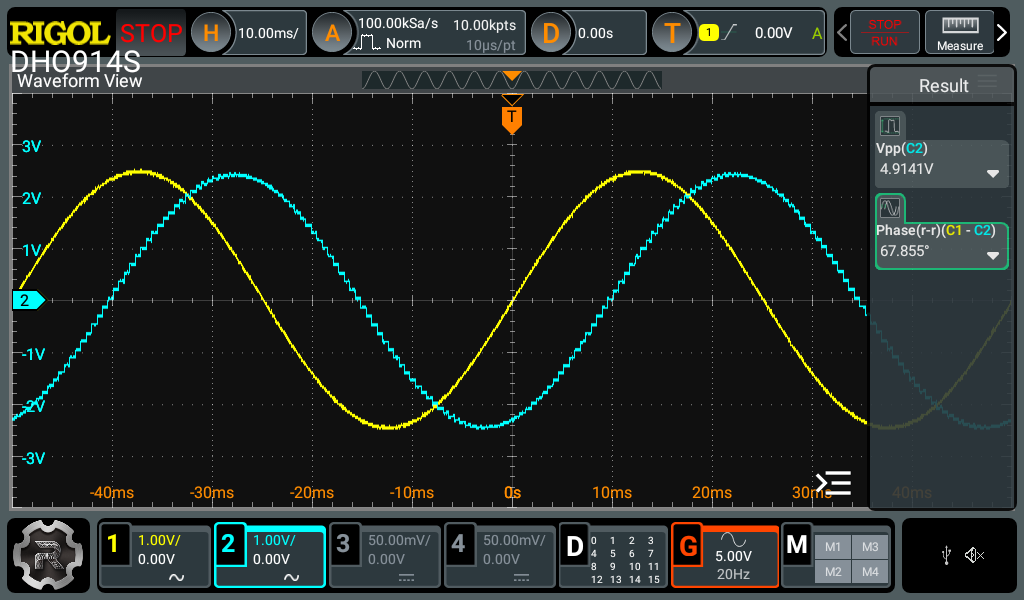
\includegraphics[width=.98\linewidth]{figures/L6_5_20Hz0.png}
	\caption{Frequency-response measurement at $20\,\text{Hz}$: \texttt{Vpp(C2)} $=4.9141\,\text{V}$, \texttt{Phase(r-r)(C1-C2)} $=67.855^{\circ}$.}
	\label{fig:L65_20}
\end{figure}

\begin{figure}[htb]
	\centering
	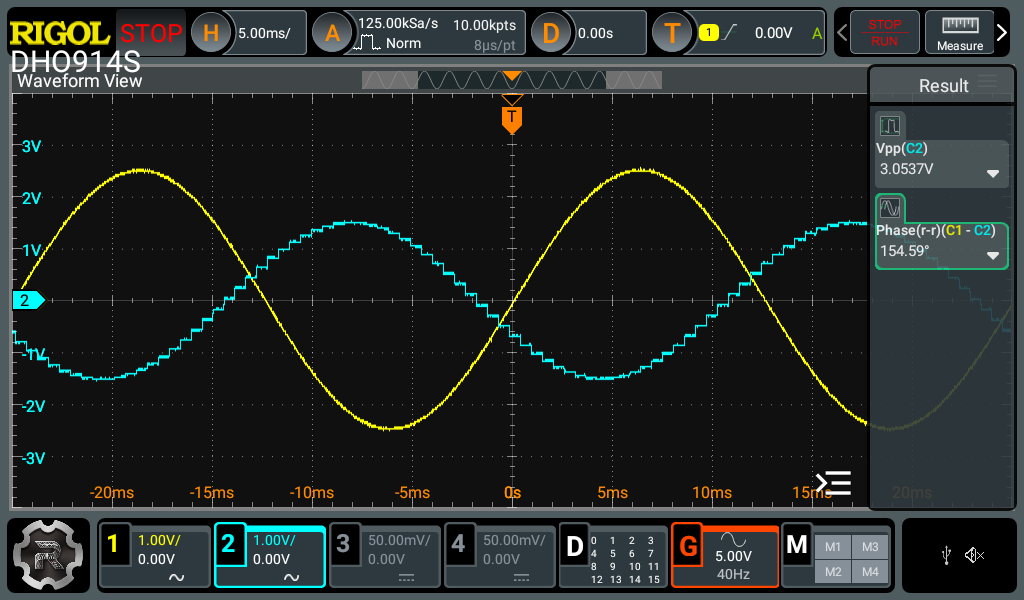
\includegraphics[width=.98\linewidth]{figures/L6_5_40Hz0.png}
	\caption{Frequency-response measurement at $40\,\text{Hz}$: \texttt{Vpp(C2)} $=3.0537\,\text{V}$, \texttt{Phase(r-r)(C1-C2)} $=154.59^{\circ}$.}
	\label{fig:L65_40}
\end{figure}

\begin{figure}[htb]
	\centering
	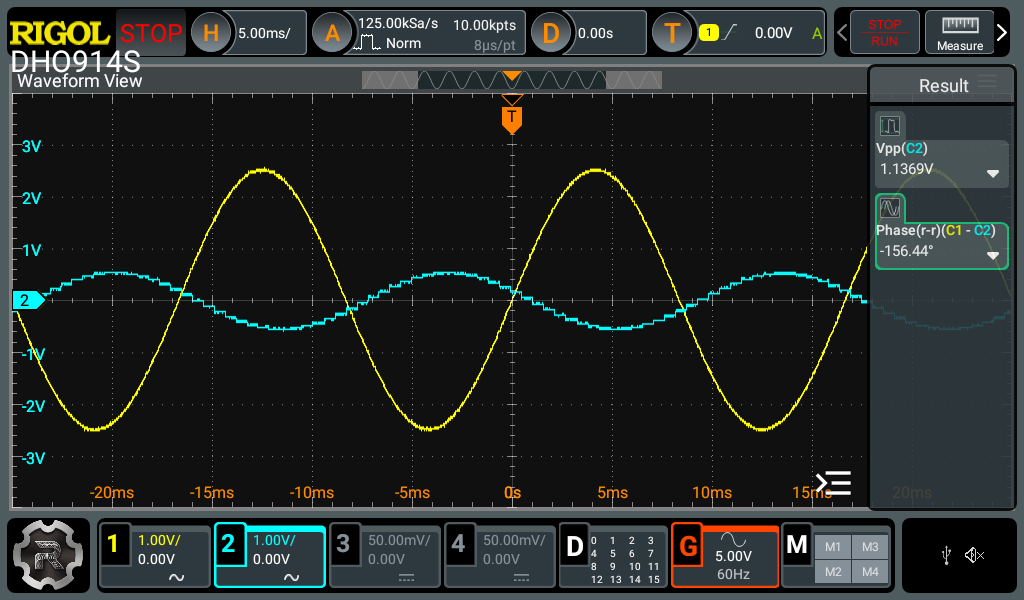
\includegraphics[width=.98\linewidth]{figures/L6_5_60Hz0.png}
	\caption{Frequency-response measurement at $60\,\text{Hz}$: \texttt{Vpp(C2)} $=1.1369\,\text{V}$, \texttt{Phase(r-r)(C1-C2)} $=-156.44^{\circ}$.}
	\label{fig:L65_60}
\end{figure}

\begin{figure}[htb]
	\centering
	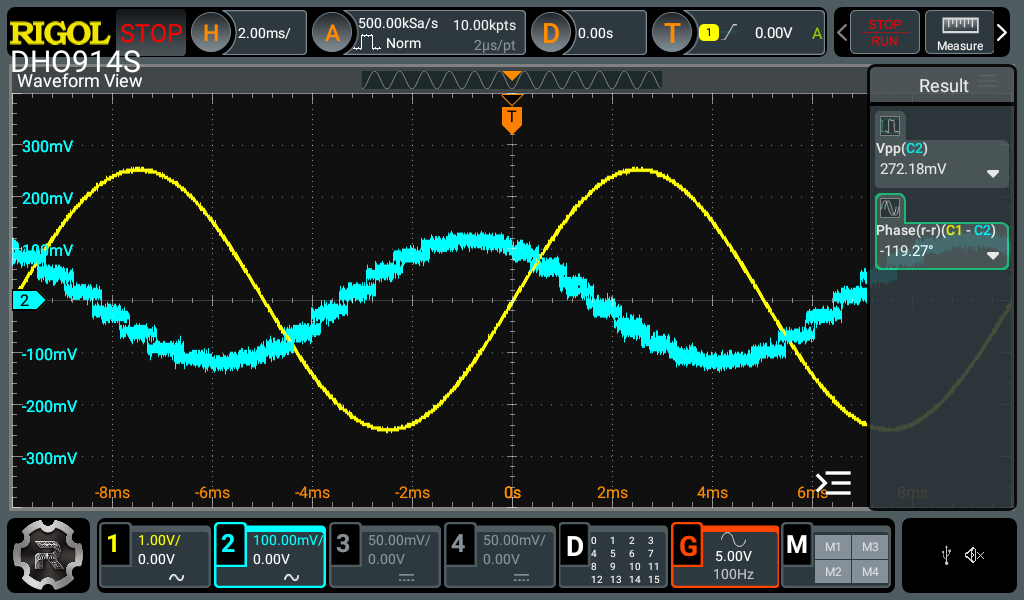
\includegraphics[width=.98\linewidth]{figures/L6_5_100Hz0.png}
	\caption{Frequency-response measurement at $100\,\text{Hz}$: \texttt{Vpp(C2)} $=272.18\,\text{mV}$, \texttt{Phase(r-r)(C1-C2)} $=-119.27^{\circ}$.}
	\label{fig:L65_100}
\end{figure}

\begin{figure}[htb]
	\centering
	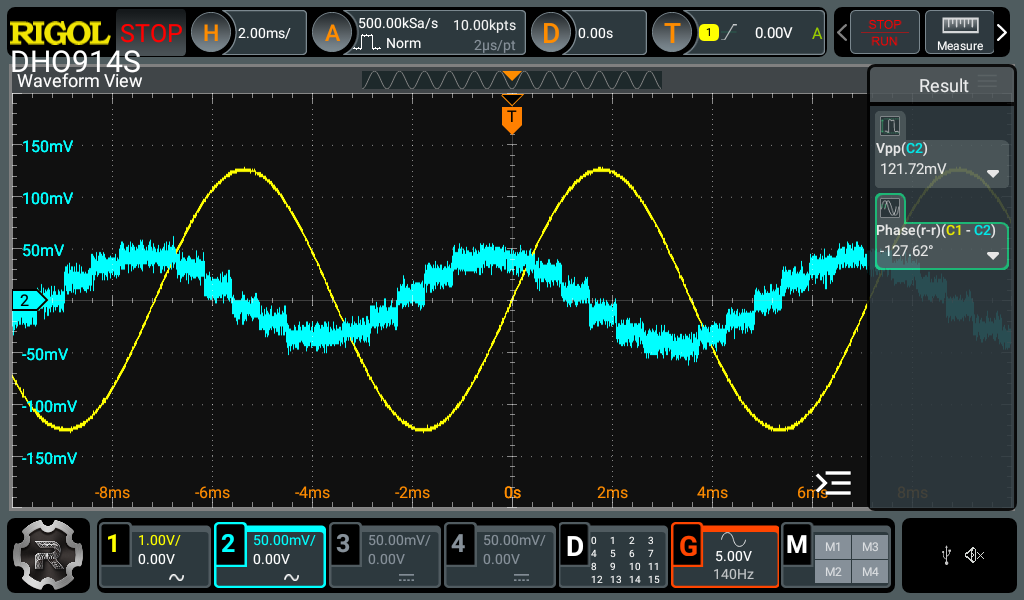
\includegraphics[width=.98\linewidth]{figures/L6_5_140Hz0.png}
	\caption{Frequency-response measurement at $140\,\text{Hz}$: \texttt{Vpp(C2)} $=121.72\,\text{mV}$, \texttt{Phase(r-r)(C1-C2)} $=-127.62^{\circ}$.}
	\label{fig:L65_140}
\end{figure}

\begin{figure}[htb]
	\centering
	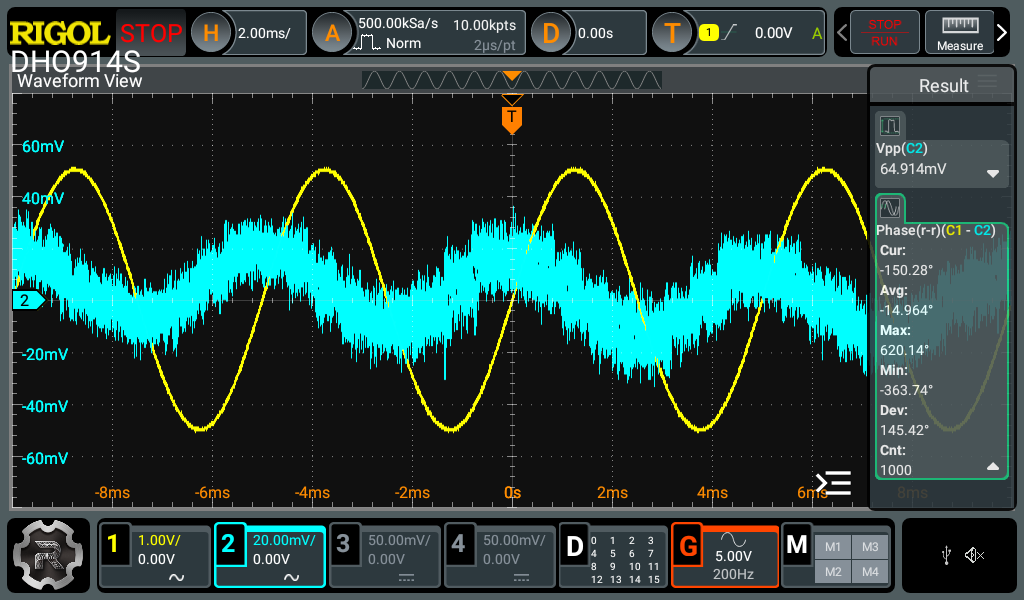
\includegraphics[width=.98\linewidth]{figures/L6_5_200Hz0.png}
	\caption{Frequency-response measurement at $200\,\text{Hz}$: \texttt{Vpp(C2)} $=64.914\,\text{mV}$, \texttt{Phase(r-r)(C1-C2)} current value $=-150.28^{\circ}$ (phase display fluctuates at this low-amplitude, high-noise condition).}
	\label{fig:L65_200}
\end{figure}

\subsection{Problem L6.6}
From the data collected in Problem L6.5, compute the transfer-function magnitude in decibels at each tested frequency.

\vspace{\baselineskip}
<findings>

\section{Author Contributions}

There is only one author for this report and lab.



%%% References -------------------------

\bibliographystyle{plainnat}
\bibliography{report}

%%% Appendices -------------------------

\end{document}  